\section{Thuật toán Raita}

\subsection{Đặc điểm chính}

Thuật toán Raita là một biến thể thực nghiệm dựa trên cách dịch chuyển của thuật toán Horspool. Điểm khác biệt chính của thuật toán nằm ở thứ tự so sánh ký tự trong mỗi lần thử. Thay vì so sánh toàn bộ mẫu ngay từ đầu, Raita kiểm tra trước một số vị trí có khả năng loại bỏ nhanh các trường hợp không khớp.

Cụ thể, thuật toán lần lượt so sánh ký tự cuối, ký tự đầu và ký tự giữa của mẫu với các ký tự tương ứng trong cửa sổ văn bản. Chỉ khi cả ba phép so sánh này đều khớp, thuật toán mới tiếp tục so sánh các ký tự còn lại.

Thuật toán có các đặc điểm sau:

\begin{itemize}
    \item trước hết so sánh ký tự cuối của mẫu, sau đó đến ký tự đầu, rồi ký tự giữa, trước khi so sánh các ký tự còn lại;
    \item thực hiện phép dịch chuyển giống thuật toán Horspool;
    \item giai đoạn tiền xử lý có độ phức tạp thời gian \(O(m+\sigma)\) và không gian \(O(\sigma)\);
    \item giai đoạn tìm kiếm có độ phức tạp thời gian \(O(mn)\).
\end{itemize}

\subsection{Mô tả thuật toán}

Raita đã thiết kế một thuật toán trong đó, tại mỗi lần thử, thuật toán đầu tiên so sánh ký tự cuối của mẫu với ký tự ngoài cùng bên phải của cửa sổ văn bản. Nếu hai ký tự này khớp, thuật toán tiếp tục so sánh ký tự đầu tiên của mẫu với ký tự ngoài cùng bên trái của cửa sổ. Nếu tiếp tục khớp, thuật toán so sánh ký tự ở giữa mẫu với ký tự tương ứng ở giữa cửa sổ văn bản.

Cuối cùng, nếu cả ba phép so sánh trên đều khớp, thuật toán mới thực sự so sánh các ký tự còn lại, từ ký tự thứ hai đến ký tự áp chót. Trong quá trình này, ký tự ở giữa có thể được so sánh lại.

Raita quan sát rằng thuật toán của mình có hiệu năng tốt trong thực tế khi tìm kiếm mẫu trong văn bản tiếng Anh, và cho rằng hiệu năng này đến từ sự phụ thuộc giữa các ký tự. Tuy nhiên, Smith đã thực hiện thêm một số thí nghiệm và kết luận rằng hiện tượng này có thể chủ yếu đến từ ảnh hưởng của trình biên dịch.

Giai đoạn tiền xử lý của thuật toán Raita bao gồm việc tính hàm dịch chuyển bad-character như trong thuật toán Boyer-Moore. Giai đoạn này có thể được thực hiện với độ phức tạp thời gian \(O(m+\sigma)\) và độ phức tạp không gian \(O(\sigma)\).

Giai đoạn tìm kiếm của thuật toán Raita có độ phức tạp thời gian bậc hai trong trường hợp xấu nhất.

\subsection{Cài đặt bằng C++}
\begin{verbatim}
#include <iostream>
#include <vector>
#include <string>
#include <cstring>

using namespace std;

const int ASIZE = 256;

/* Bad Character Shift Table */
void preBmBc(const string &pat, vector<int> &bmBc) {
    int m = pat.length();

    bmBc.assign(ASIZE, m);

    for (int i = 0; i < m - 1; ++i) {
        bmBc[(unsigned char)pat[i]] = m - 1 - i;
    }
}

/* Raita Algorithm */
void Raita(const string &pat, const string &txt) {
    int m = pat.length();
    int n = txt.length();

    if (m == 0 || n < m) {
        return;
    }

    vector<int> bmBc;

    /* Preprocessing */
    preBmBc(pat, bmBc);

    char firstCh = pat[0];
    char middleCh = pat[m / 2];
    char lastCh = pat[m - 1];

    /* Searching */
    int j = 0;

    while (j <= n - m) {
        unsigned char c = (unsigned char)txt[j + m - 1];

        if (lastCh == txt[j + m - 1] &&
            middleCh == txt[j + m / 2] &&
            firstCh == txt[j] &&
            memcmp(pat.c_str() + 1, txt.c_str() + j + 1, m - 2) == 0) {
            cout << "Pattern found at index: " << j << endl;
        }

        j += bmBc[c];
    }
}

int main() {
    string text = "ABAAABCDABCABC";
    string pattern = "ABC";

    Raita(pattern, text);

    return 0;
}
\end{verbatim}

\subsection{Kiểm nghiệm thuật toán}

\textbf{Pha tiền xử lý:}

\begin{center}
    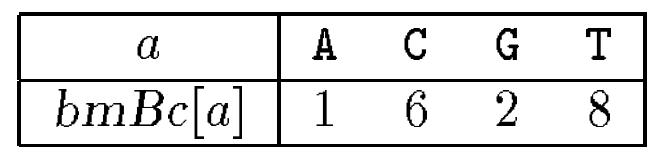
\includegraphics[width=10cm]{Images/2026-05-18-15-59-23.png}
\end{center}

Bảng $bmBc$ được sử dụng bởi thuật toán Raita.

\textbf{Pha tìm kiếm:}

Lần 1:

\begin{center}
    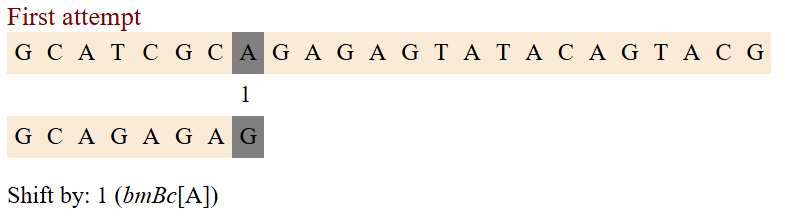
\includegraphics[width=15cm]{Images/2026-05-18-16-00-26.png}
\end{center}

Lần 2:

\begin{center}
    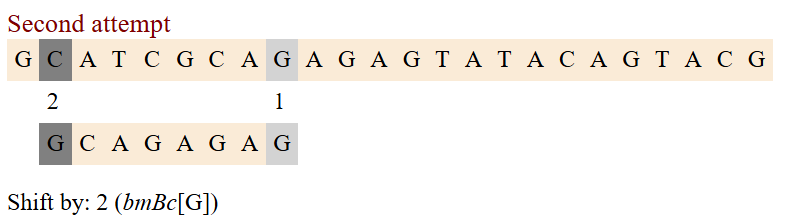
\includegraphics[width=15cm]{Images/2026-05-18-16-00-38.png}
\end{center}

Lần 3:

\begin{center}
    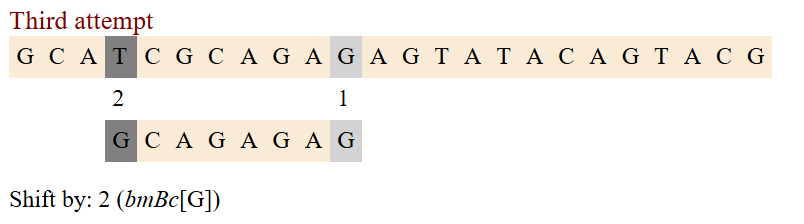
\includegraphics[width=15cm]{Images/2026-05-18-16-00-49.png}
\end{center}

Lần 4:

\begin{center}
    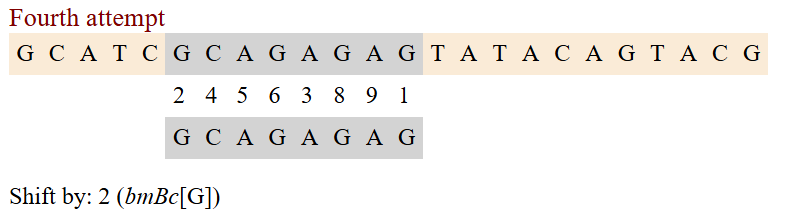
\includegraphics[width=15cm]{Images/2026-05-18-16-01-11.png}
\end{center}

Lần 5:

\begin{center}
    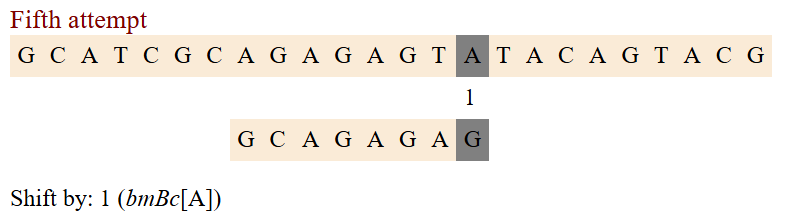
\includegraphics[width=15cm]{Images/2026-05-18-16-01-24.png}
\end{center}

Lần 6:

\begin{center}
    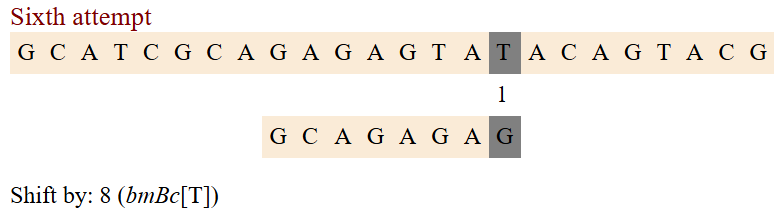
\includegraphics[width=15cm]{Images/2026-05-18-16-01-32.png}
\end{center}

Lần 7:

\begin{center}
    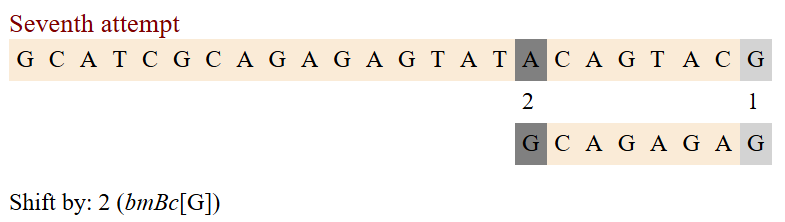
\includegraphics[width=15cm]{Images/2026-05-18-16-02-11.png}
\end{center}

Thuật toán Raita thực hiện 18 lần so khớp chuỗi trong ví dụ trên.